%%%%%%%%%%%%%%%%%%%%%%%%%%%%%%%%%%%%%%%%%
% MUW Poster
% LaTeX Template
% Version 1.0 (31/08/2016)
% (Based on Version 1.0 (31/08/2015) of the Jacobs Portrait Poster
%
% License:
% CC BY-NC-S3.0 (http://creativecommons.org/licenses/by-nc-sa/3.0/)
%
% Created by:
% Nicolas Ballarini, CeMSIIS, Medical University of Vienna
% nicoballarini@gmail.com
% http://statistics.msi.meduniwien.ac.at/
%%%%%%%%%%%%%%%%%%%%%%%%%%%%%%%%%%%%%%%%%


\def\footer#1{\def\insertfooter{#1}}
% --------------------------------------------------------------------------------------
%	PACKAGES AND OTHER DOCUMENT CONFIGURATIONS
% --------------------------------------------------------------------------------------

\documentclass[final]{beamer}

\usepackage[scale=1.09]{beamerposter} % Use the beamerposter package


% Include a logo of your project if desired
% \logo{\pgfputat{\pgfxy(-6,93)}{\pgfbox[center,base]{
\includegraphics[width=0.15\textwidth]{ProjectLogo.jpg}}}}

\usepackage{multicol}
\usepackage[utf8]{inputenc}
\usepackage{array}
% The following two are column definitions for the aknowledgements section
\newcolumntype{L}{>{\arraybackslash}m{22cm}}
\newcolumntype{S}{>{\arraybackslash}m{5cm}}
\usepackage{pgf}
\usepackage{mathtools}
\usepackage{amsmath, amsthm, amssymb, amsfonts, empheq}
\usepackage{exscale}
\usepackage{xcolor}
\usepackage{ushort}
\usepackage{setspace}
\usepackage[square,numbers]{natbib}
\usepackage{url}
\usepackage{multirow}
\usepackage{arydshln}
\usepackage{ragged2e} % Justify text
\addtobeamertemplate{block begin}{}{\justifying} % Justify all blocks
\renewcommand{\indent}{\hspace*{2em}}
\newtheorem{proposition}{Proposition}

\bibliographystyle{nat}
\renewcommand{\vec}[1]{\ushort{#1}}
\renewcommand{\vec}[1]{\mathbf{#1}}
\definecolor{greenMUW}{RGB}{60,191,174}
\definecolor{blueMUW}{RGB}{17,79,29}
\definecolor{skinMUW}{RGB}{234,208,207}
\definecolor{micolor}{RGB}{04,88,137}
\definecolor{hellblauMUW}{RGB}{225,133,33}
\setbeamercolor{block title}{bg=white, fg = hellblauMUW}

\setbeamercolor{alerted text}{fg=greenMUW!200}
\setbeamercolor{structured text}{fg=hellblauMUW}
% -----------------------------------------------
% START Set the colors
% Uncomment to apply colors you want to use.
% -----------------------------------------------
\colorlet{themecolor}{hellblauMUW}
% \usebackgroundtemplate{\includegraphics[width=\paperwidth]{MUW_hellblau.pdf}}

% \colorlet{themecolor}{skinMUW}
% \colorlet{themecolor}{blueMUW}
% \usebackgroundtemplate{\includegraphics{MUW_skin.pdf}}

%% \colorlet{themecolor}{blueMUW}
% \colorlet{themecolor}{hellblauMUW}
% \usebackgroundtemplate{\includegraphics{MUW_hellblau.pdf}}
% -----------------------------------------------
% END Set the colors
% -----------------------------------------------


% -----------------------------------------------
% START Set the width of the columns
% -----------------------------------------------
\setlength{\paperwidth}{90cm} % A0 width: 46.8in
\setlength{\paperheight}{110cm} % A0 height: 33.1in
\newlength{\sepmargin}
\newlength{\sepwid}
\newlength{\onecolwid}
\newlength{\twocolwid}
\newlength{\threecolwid}

% The following measures are used for 2 columns
\setlength{\sepmargin}{0.055\paperwidth} % Separation width (white space) between columns
\setlength{\sepwid}{0.03\paperwidth} % Separation width (white space) between columns
\setlength{\onecolwid}{0.43\paperwidth} % Width of one column
\setlength{\twocolwid}{0.9\paperwidth} % Width of two columns

% -----------------------------------------------------------
% The following measures are used for 3 columns
% \setlength{\sepmargin}{0.06\paperwidth} % Separation width (white space) between columns
% \setlength{\sepwid}{0.02\paperwidth} % Separation width (white space) between columns
% \setlength{\onecolwid}{0.28\paperwidth} % Width of one column
% \setlength{\twocolwid}{0.58\paperwidth} % Width of two columns
% \setlength{\threecolwid}{0.88\paperwidth} % Width of three columns
% \setlength{\columnsep}{30pt}

% -----------------------------------------------
% END Set the width of the columns
% -----------------------------------------------


% --------------------------------------------------------------------------------------
%	TITLE SECTION
% --------------------------------------------------------------------------------------
\setbeamertemplate{title}[left]
\setbeamertemplate{frametitle}[default][left]
% \setmainfont{Georgia}

\title{Numerical schemes for Classical\\  Chemotaxis Equations  PC-239} % Poster title

% \subtitle{IX International Congress on Industrial and Applied Mathematics \\ Valencia, Spain, 15-19th July 2019}
\author{ Daniel Acosta Soba$^1$, Alba M. Navarro Izquierdo$^2$, J. Rafael Rodr\'iguez Galv\'an$^3$} % Author(s)

\institute{Departamento de Matem\'aticas, Universidad de C\'adiz} % Institution(s)
% --------------------------------------------------------------------------------------
\pagenumbering{gobble}

\usepackage{scrpage2}
\usepackage{tikz}
\usetikzlibrary{calc}
\newcommand{\pageframe}{%
  \begin{tikzpicture}[remember picture, overlay]
    % page frame
    \fill [themecolor] (current page.north west)
    rectangle (current page.south east);
    \fill [white, rounded corners=1cm] ($(current page.north west)+(1cm,-2cm)$)
    rectangle ($(current page.south east)+(-1cm,2cm)$);
    % \strut gives all page mark nodes the same hight.
    \node[inner sep=0pt] (russell) at ($(current page.north east)+(-11cm,-11cm)$)
    {
\includegraphics[width=.15\textwidth]{ProjectLogo.jpg}};
  \end{tikzpicture}

}
% set page style
\cehead[\pageframe]{\pageframe}
\cohead[\pageframe]{\pageframe}
\pagestyle{scrheadings}

\usepackage{hydstokes-sipdg}
\newcommand{\property}[1]{\alert{\textbf{#1}}}
%%%%%%%%%%%%%%%%%%%%%%%%%%%%%%%%%%%%%%%%%%%%%%%%%%%%%%%%%%%%%%%%%%%%%%%%%%%%%%

\begin{document}

\addtobeamertemplate{block end}{}{\vspace*{1ex}} % White space under blocks
\addtobeamertemplate{block alerted end}{}{\vspace*{0ex}} % White space under highlighted (alert) blocks
\setlength{\belowcaptionskip}{2ex} % White space under figures
\setlength\belowdisplayshortskip{1ex} % White space under equations


\begin{frame}[t] % The whole poster is enclosed in one beamer frame

  \begin{columns}[t]
    \begin{column}{\sepmargin}\end{column}

    \begin{column}{0.97\linewidth}
      \vskip2cm
      \raggedright
      \usebeamercolor{title in headline}{\color{blueMUW}\Huge{\textbf{\inserttitle}}\\[1.5ex] \par}
      \usebeamercolor{author in headline}{\color{blueMUW}\LARGE{\insertauthor}\\[1ex]}
      \usebeamercolor{institute in headline}{\color{blueMUW}\normalsize{\insertinstitute}}{\color{blueMUW}}
      \vspace*{0.5cm}

      \rule{1.012\textwidth}{10pt}
    \end{column}
  \end{columns}

  \vspace*{0.5cm}

  \begin{columns}[t] % The whole poster consists of two major columns

    \begin{column}{\sepmargin}\end{column}

    \begin{column}{\onecolwid} % The first column


      \begin{block}{Introduction}
        Chemotaxis (movement of biological cells in response to
        chemical signals) was modeled by Keller-Segel in 1970.
        Although there are several models, we focus on the
        classical one, given by the following equations in
        $\Omega\subset\mathbb{R}^n$:
        \begin{subequations}\label{KSclasico}
          \begin{empheq}[left=\empheqlbrace]{align}
            &u_t= \alpha_0\Delta u - \alpha_1\nabla\cdot( u\nabla v), \quad \xx\in\Omega,\, t>0, \label{KSclasico:a}\\
            &v_t= \alpha_2\Delta v -\alpha_3 v+\alpha_4 u,  \quad \xx\in\Omega,\, t>0,\label{KSclasico:b}\\[0.2cm]
            &\grad u \cdot \nn = \grad v \cdot \nn = 0, \quad \xx\in\partial\Omega,\, t>0, \\[0.2cm]
            &u(\xx,0)=u_0(\xx), \enspace v(\xx,0)=v_0(\xx), \quad \xx\in\Omega,
          \end{empheq}
        \end{subequations}
        where $u$ and $v$ represent density of
        \alert{cells} and \alert{chemical-signal}, respectively.

        \bigskip\par\indent From an analytical point of view, a lot of
        research has been recently done (see e.g.~\cite{Winkler} and
        references therein) and interesting results about global in time
        existence, \alert{mass conservation}, \alert{energy}, blow-up and
        \alert{positivity of solution} have been published.  However,
        there is not a large literature on \textit{numerical analysis}
        for~(\ref{KSclasico}), and reproducing former properties is an
        interesting challenge. This work is mainly focused on development
        of \textit{positivity preserving numerical schemes}, related to
        discontinuous \textit{Galerkin methods}, which \textit{decouple}
        calculus of $u$ and $v$.

      \end{block}

      \begin{block}{Energy-Stable Semi-Discretization in Time}
        Given a partition of time interval $(0,T)$ into subintervals
        of size $k>0$, we approximate $u$ and $v$ at each time step
        $t^{m+1}$ by an implicit Euler scheme\footnote{However,
          this work can be applied to higher order implicit methods
          or, following \cite{anderson_high-order_2017} and references
          therein, to parallel explicit high-order approximations via
          Strong Stability Preserving (SSP) methods} as follows:
        \begin{subequations}\label{tfgschemes}
          \begin{empheq}[left=\empheqlbrace]{align}
            &\delta_t v^{m+1}-\alpha_2\nabla v^{m+s}+\alpha_3v^{m+s}-\alpha_4u^{m}=0, \label{TFGschemes:b} \\
            &\delta_t u^{m+1}-\alpha_0\Delta u^{m+s} +\alpha_1\nabla\cdot(u^{m+s}\nabla v^{m+s})=0,\label{TFGschemes:a}
          \end{empheq}
        \end{subequations}
        where $s\in\{0,1\}$ and $\delta_t$ is the backward difference
        operator. For this schemes, \property{energy-stability} (for
        an adequate discrete energy functional) can be shown~\cite{Alba_TFG}.
      \end{block}

      \begin{block}{Space Discretization for~(\ref{TFGschemes:a})}
        Let $\Th$ be a mesh of $\Omega$ and we define
        $\Uh=\{\phi\in
        L^2(\Omega)\colon\phi|_K\in\mathbb{P}_k(K),\forall
        K\in\mathcal{T}_h \}$ where $\mathbb{P}_k(K)$ is a polynomial
        space over the element $K\in\Th$. Let
        $\{\phi_1,\ldots,\phi_N\}$ be a basis of $U_h$, where
        $N=\text{dim}(U_h)$. We fix\footnote{Results presented here
          might be improved to high order space approximations by
          using Bernstein polynomials,
          see\cite{anderson_high-order_2017}} $k=1$.

        \bigskip\par\indent Let $\Vh$ be an
        space of (conforming or not) FE. For each, $m\ge 0$ we compute
        $\vmm\in\Vh$ from~(\ref{TFGschemes:b}), where the discontinuous function $\um\in\Uh$
        is replaced by $P_{\Vh}(\um)$, its $L^2(\Omega)$--projection
        on $\Vh$. Then we define $\wwmm = \grad \vmm \in \Uh^2$.

        \bigskip\par\indent Let us consider the following discrete problem: find
        $\umm\in\Uh$ such that
        \begin{equation}
          \label{discrete_problem_u}
          \int_\Omega \delta_t\umm \phi + \asip(\umm,\phi) + \agod(\umm,\phi)=0 \quad \forall\phi\in\Uh,
        \end{equation}
        where
        \begin{align*}
          \asip(u,\phi) &= \sum_{K\in\mathcal{T}_h}\int_K\nabla_h u\nabla_h \phi-\sum_{e\in\mathcal{E}_h}\int_e\left(\average{\nabla_h u\cdot\mathbf{n}_e}\jump{\phi}+\average{\nabla_h \phi\cdot\mathbf{n}_e}\jump{u}\right)\\&+\sigma\sum_{e\in\mathcal{E}_h}\int_e\frac{1}{h_e}\jump{u}\jump{\phi},
          \\
          \agod(u,\phi) &= -\sum_{K \in\mathcal{T}_h} \int_K u \, (\wwmm\cdot \grad\phi)
                          + \sum_{e\in\Eh}\{ u \, \wwmm \cdot \nn_e\}_\star
        \end{align*}
        and
        $$
        \{ u \, \wwmm \cdot \nn_e\}_\star=(\wwmm\cdot \nn_e)\average{u} -\frac{1}{2}|\wwmm\cdot\nn_e|\jump{u}
        $$
        is the Godunov (upwind) flux~\cite{anderson_high-order_2017}.

      \end{block}

    \end{column}



    \begin{column}{\sepwid}  \end{column}

    \vspace*{0.5cm}

    \begin{column}{\onecolwid} %The second column
      \begin{block}{Positivity for for Cell Density Equation}
        Equation~(\ref{TFGschemes:a}) can be recast, for
        $U^m=(U_i(t^m))_{i=1}^N)$ d.o.f of $\uh(\xx,t^{m})$, as:
        \medskip
        \begin{subequations}\label{matrix_eq_u}
          \begin{align}
            &M \; (\delta_t\Umm) + K\, U^{m+s} = 0, \quad \text{ where}
            \\[0.1ex]
            &M_{ij} = \int_\Omega \Phi_i\Phi_j,
            % \quad K&=D+C,
            % \quad D_{ij}=\asip(\Phi_i,\Phi_j),
            % \quad C_{ij}=\agod(\Phi_i,\Phi_j).
                       \quad K_{ij}=\asip(\Phi_i,\Phi_j)+\agod(\Phi_i,\Phi_j).
          \end{align}
        \end{subequations}
        Let us consider the system
        \begin{subequations}\label{discrete_upwinded_eq_u}
          \begin{align}
            &M^\star \; (\delta_t\Umm) + K^\star \, U^{m+s} = 0,
              \intertext{where $M^\star$ is the \alert{mass lumped} matrix and $K^\star$ is the \alert{discrete
              upwinded} matrix:}
            & K^\star = K + L, \quad L_{ij}=\max(0,-K_{ij},-K_{ji}) \enspace \text{if } i\neq j, \quad L_{ii}=-\sum_{j\neq i} L_{ij}.
          \end{align}
        \end{subequations}
        Then we conjecture the following result:
        \textbf{\alert{system~(\ref{discrete_upwinded_eq_u}) is positive}} in
        the sense that
        \begin{center}
          if $\uh^0=u_0(\xx)\ge 0$ in $\Omega$, then $\umm\ge 0$ for all $m\ge 0$.
        \end{center}
        This result can be shown in the case $s=0$ if $\div\wwm=0$ (by a
        generalization of \cite{anderson_high-order_2017}, where the fact
        that $K$ has zero row and column sums, i.e.
        $\sum_j K_{ij}=\sum_i K_{ij}=0$, is applied for small enough $k$).
        Although $\div\wwm\neq 0$ if $\wwm$ comes from $\grad \vmm$ (and
        the zero row property is not satisfied), it also would be valid
        provided $v\in L^\infty(0,T;W^{1,\infty}(\Omega))$. Numerical
        tests support positivity of $\uh$ in any case.

        \bigskip\par
        \textbf{Numerical Tests}:
        \begin{small}
          $\Omega=\{(x,y)\in \mathbb{R}^2,\ x^2+y^2< 9/4\}$,
          $u_0=v_0=10 e^{-20( x^2 + y^2 ) }$,
          $k_0=k_2=k_3=k_4=1, \alert{k_1\in\{1,2,3,4\}}$. $T=0.3$, $k=10^{-3}$,
          $h\simeq 10^{-1}$ ($60$ subintervals on $\partial\Omega$),
          implicit Euler ($s=1$).
          \begin{columns}
            \column{0.5\textwidth}
            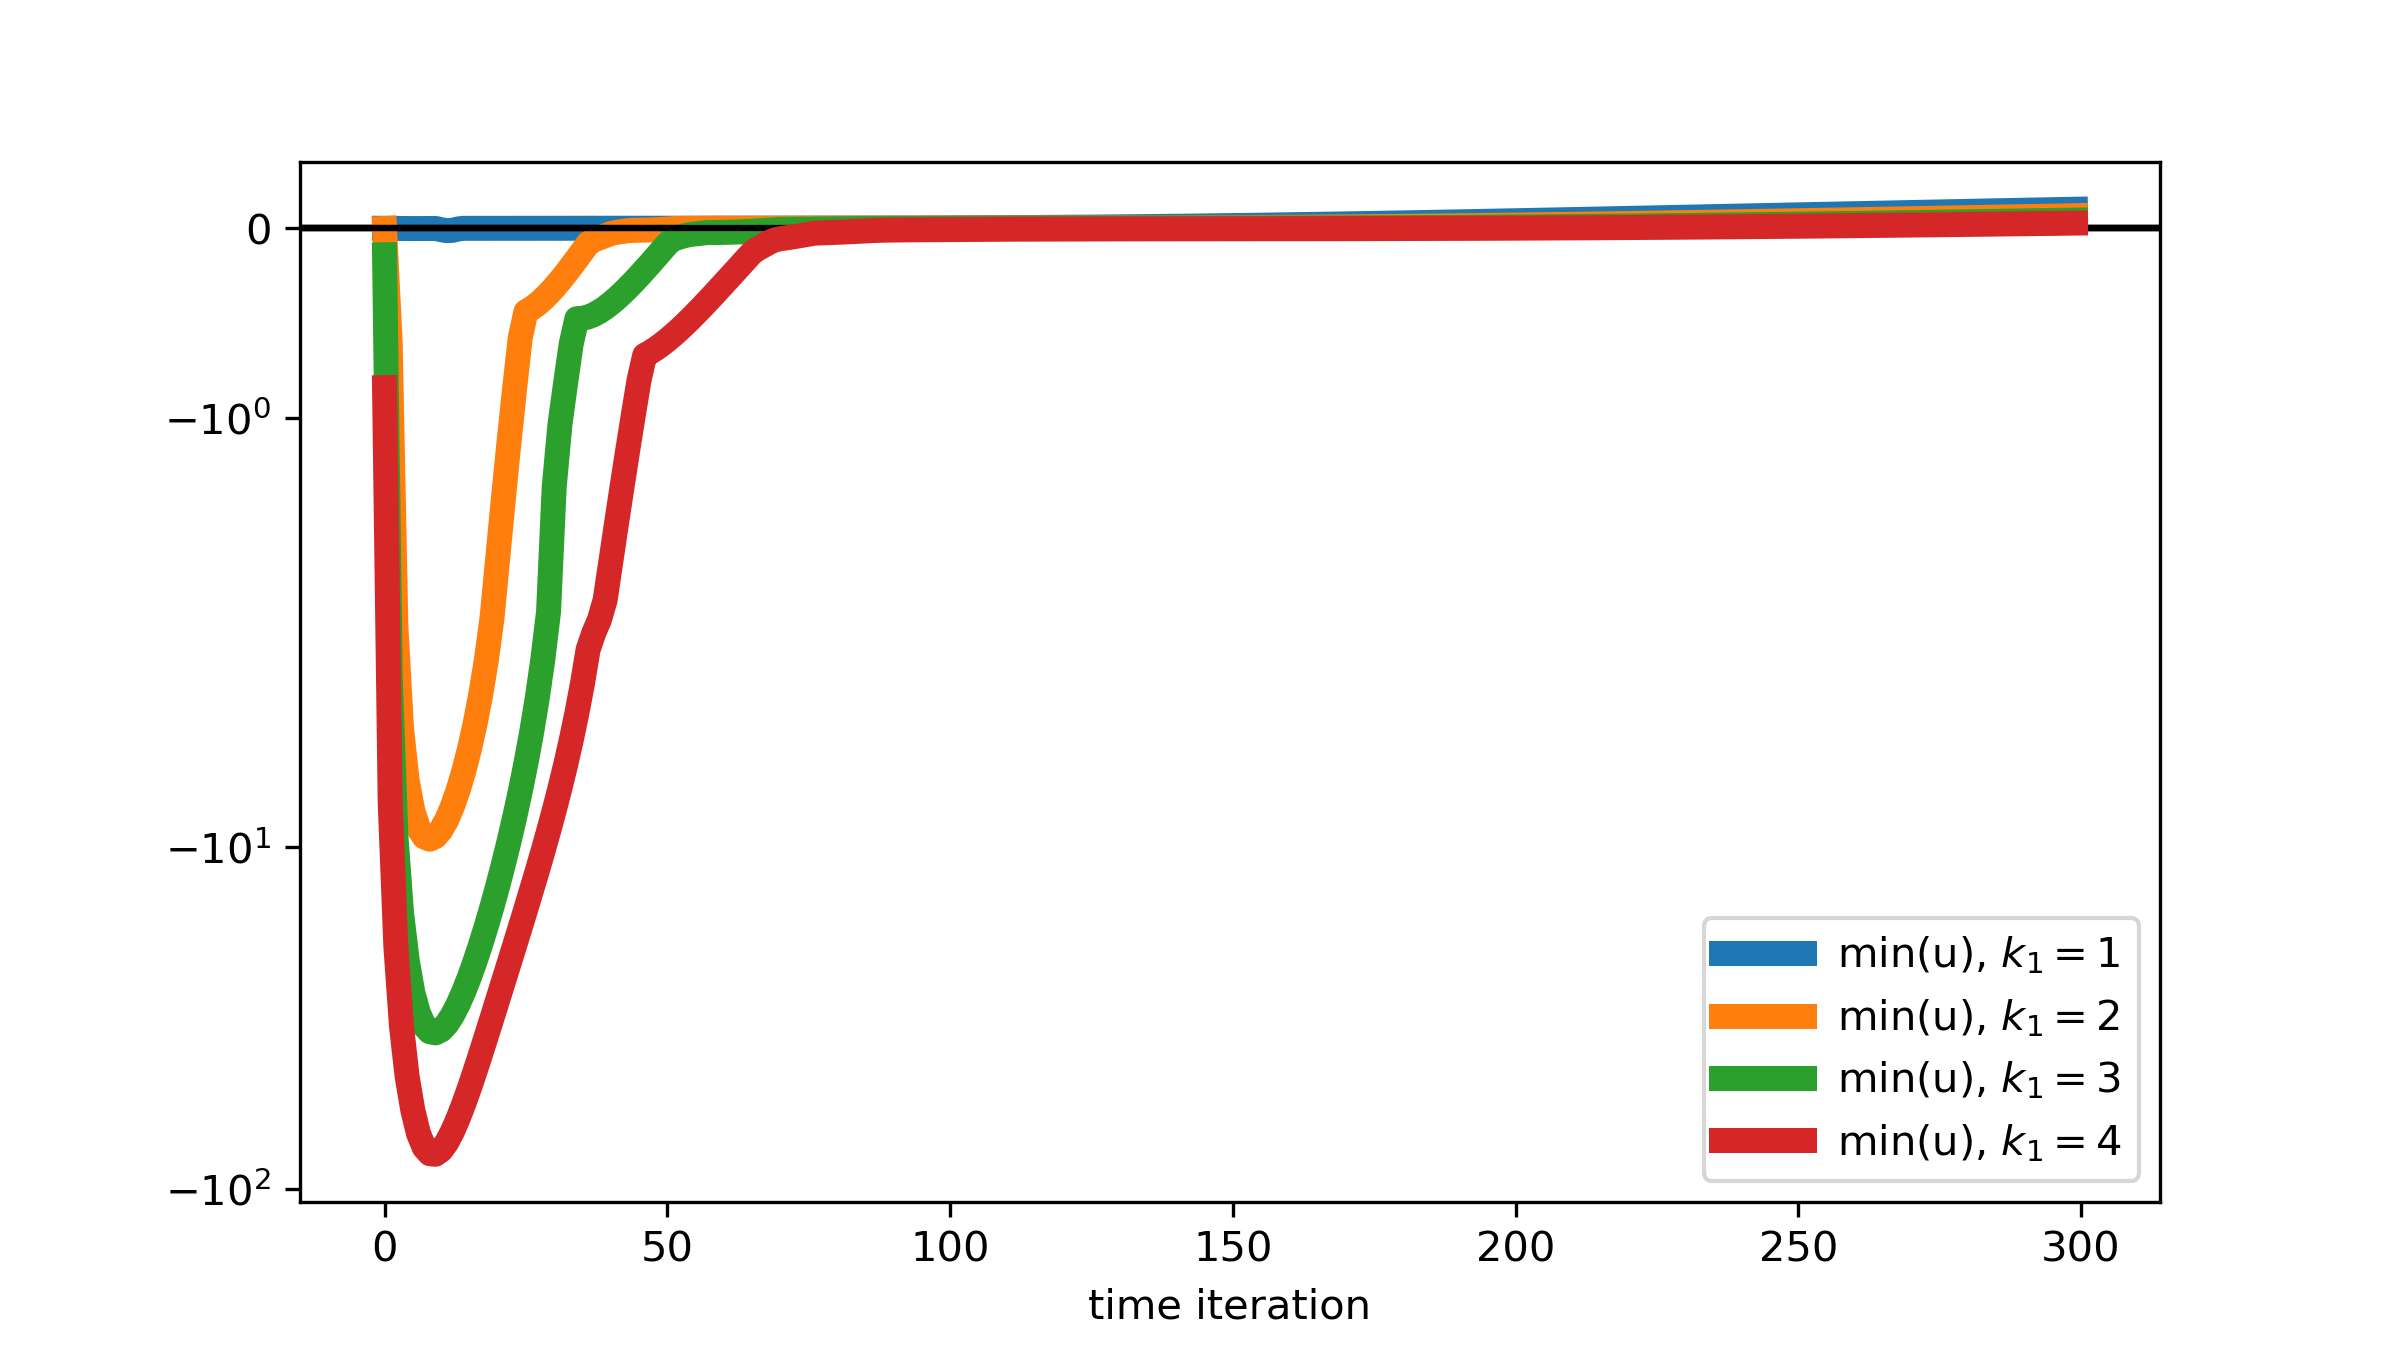
\includegraphics[width=0.9\textwidth]{negative_min_u_k1=1,2,3,4.png}
            \alert{$\mathbb{P}_1$--\textbf{continuous FE}} approximation of
            scheme~(\ref{TFGschemes:a}). \textbf{Loss of positivity}
            $\forall k_2\in\{1,2,3,4\}$.

            \column{0.5\textwidth}
            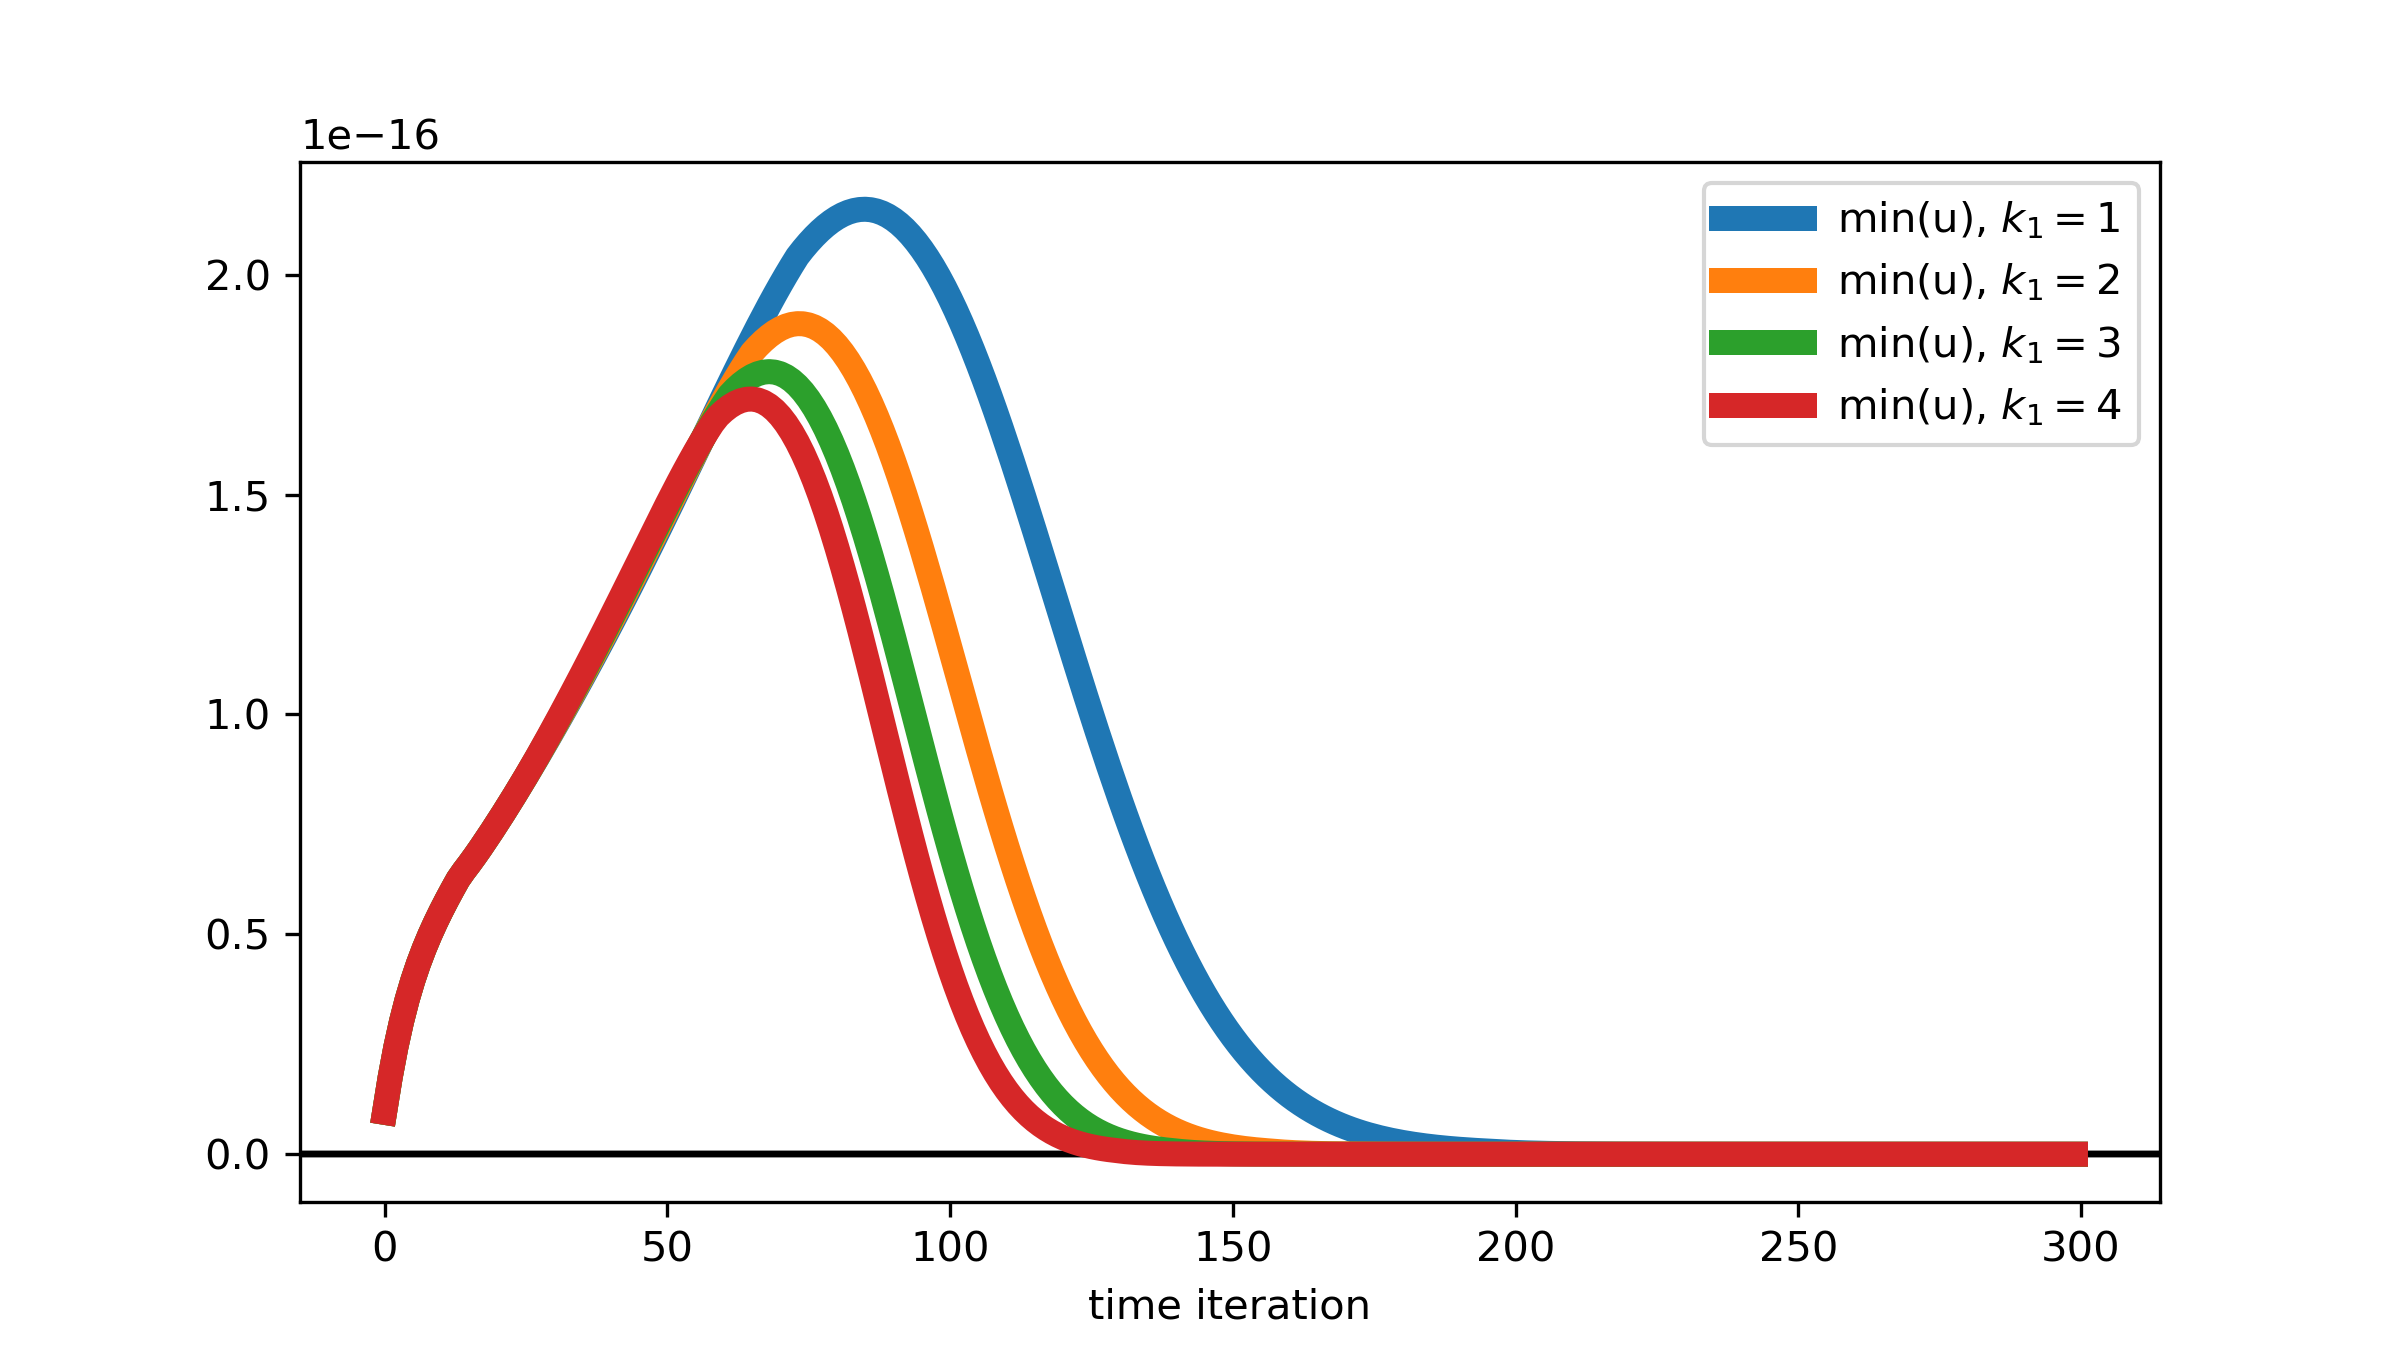
\includegraphics[width=0.9\textwidth]{positive_min_u_k1=1,2,3,4.png}
            \alert{$\mathbb{P}_1$--\textbf{discontinuous Galerkin}}
            approximation. \structure{\textbf{Positivity is
                achieved} $\forall k_2\in\{1,2,3,4\}$ !!}
          \end{columns}
        \end{small}
      \end{block}


      \vspace{0.2cm}

      \begin{block}{Mass Conservation}
          The method (\ref{discrete_problem_u}) is mass conservative in the following sense:
            $\int_\Omega \umm = \int_\Omega \uh^0$,
          what can be seen using the fact $\sum_i K_{ij}=0$. However,
          this property is \alert{not verified} by the discrete
          upwinded scheme~(\ref{discrete_upwinded_eq_u}) because, in
          the general case, $\div\wwmm\neq 0$ thus zero column sums
          property is not valid for $K$.

          \bigskip\par
          \textbf{Numerical Tests}: Approximate mass
          conservation for the explicit ($s=0$) method (left) but not
          for the implicit $(s=1)$ one (right). Same parameters than
          previous tests.
        \begin{columns}
          \column{0.5\textwidth}
          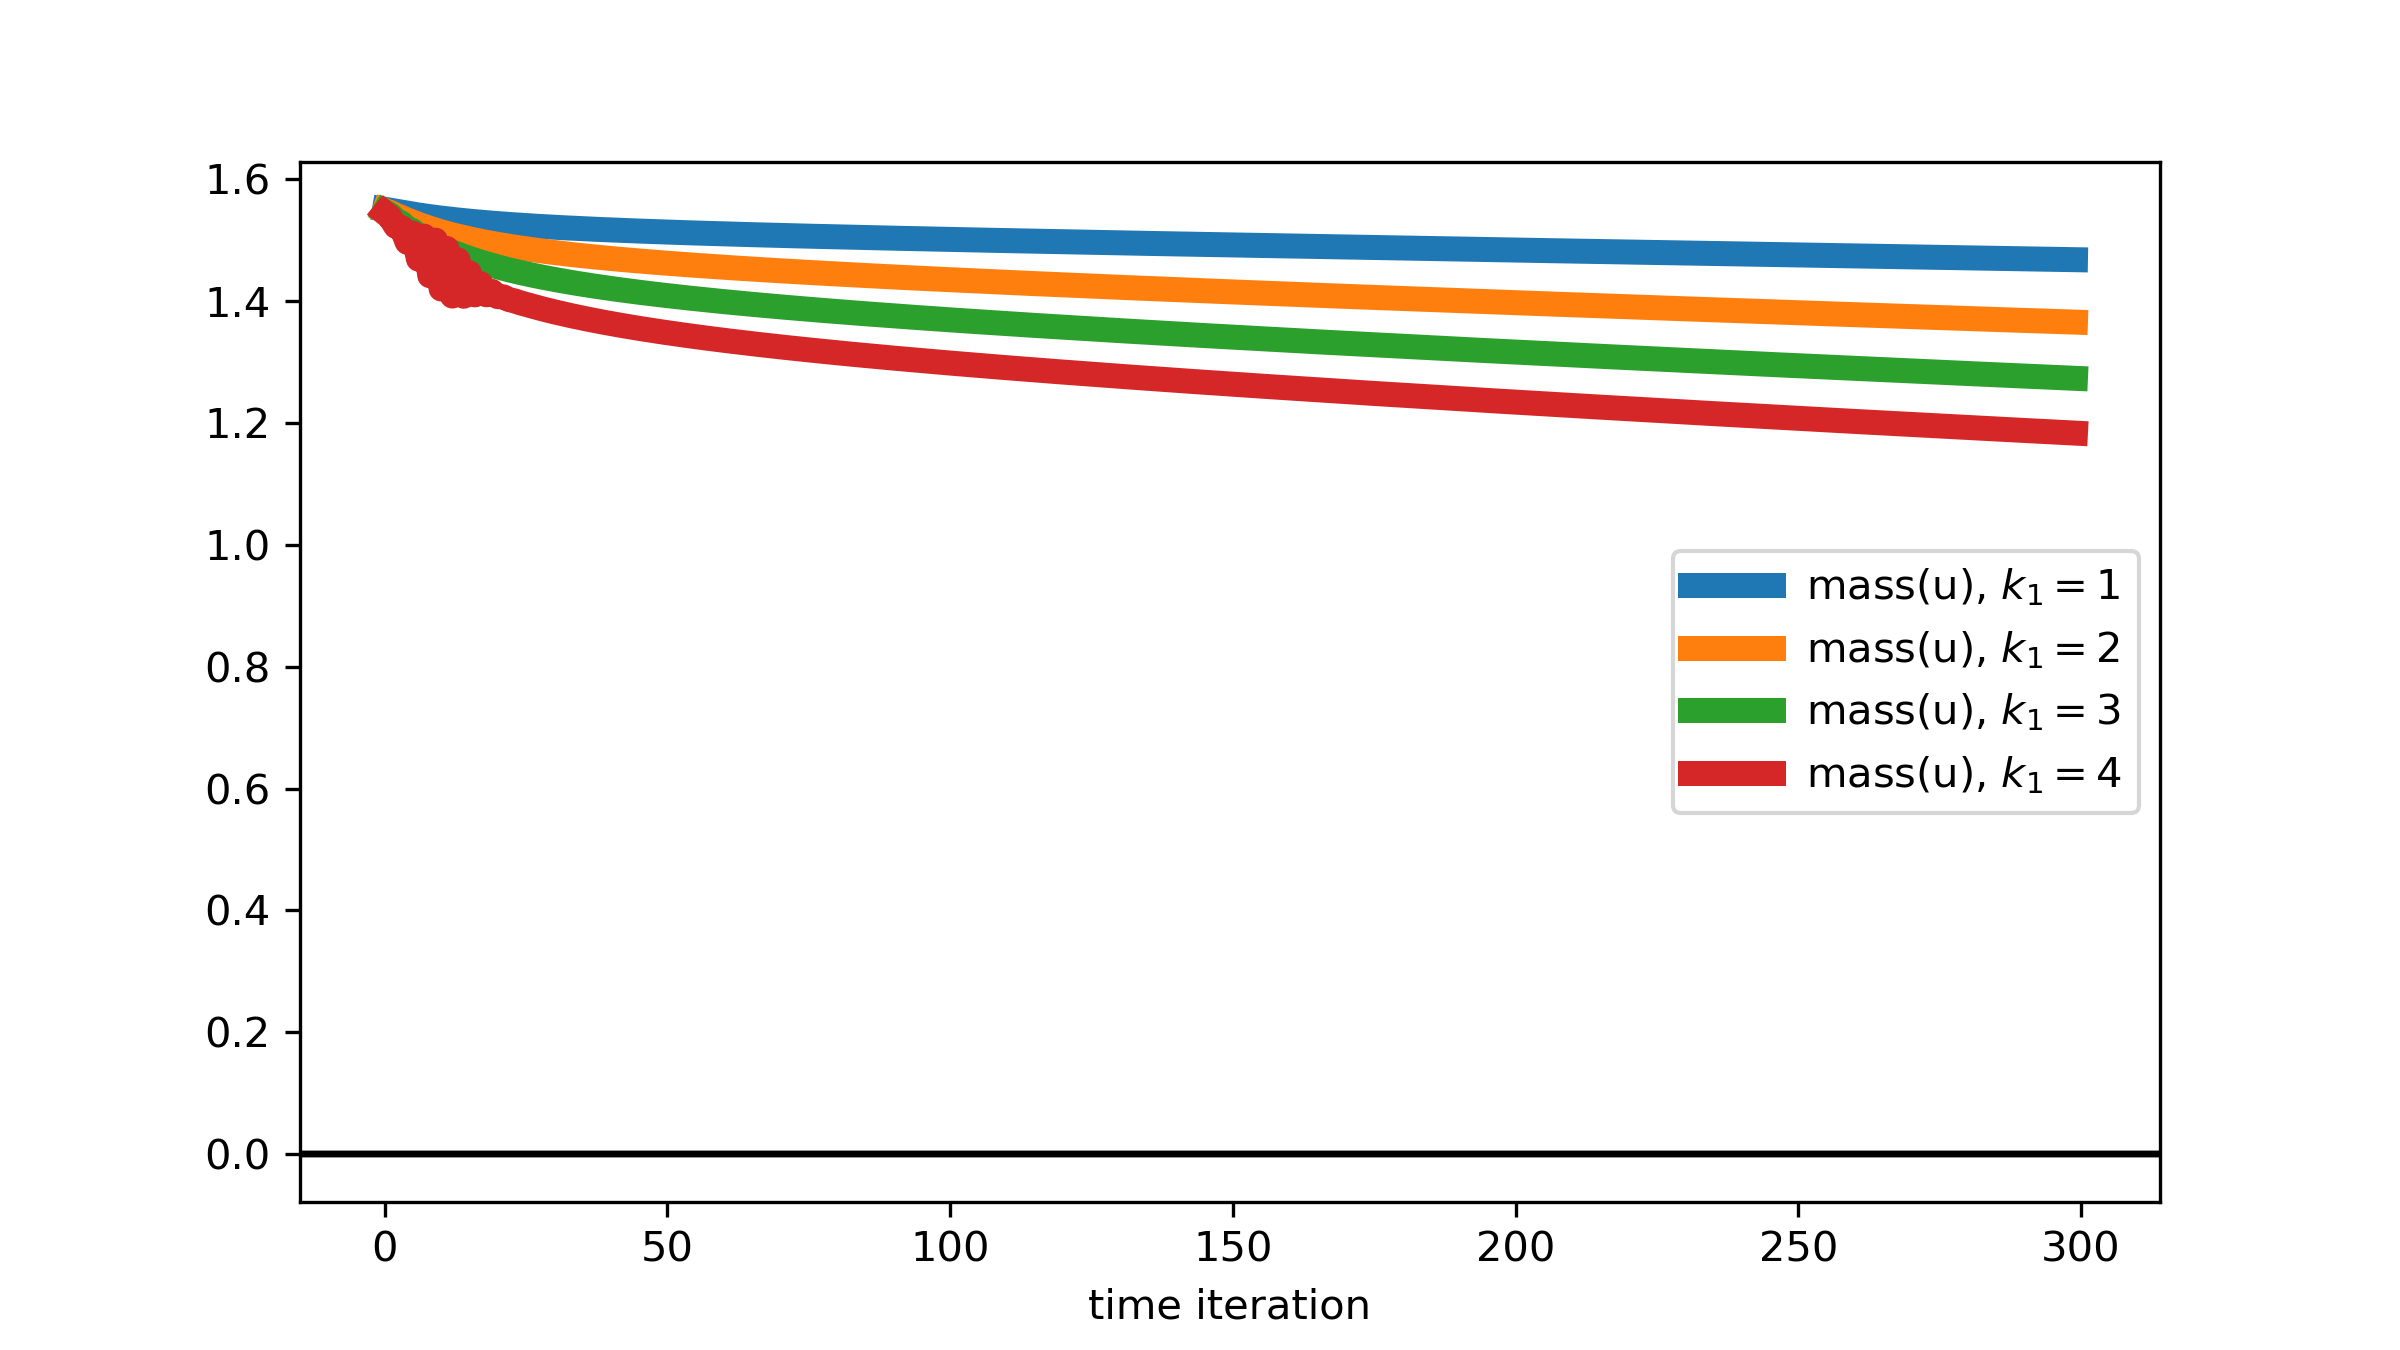
\includegraphics[width=0.8\textwidth]{positive_EXPLICIT_scheme_mass_k1=1,2,3,4.png}
          \par
          \small \alert{Explicit} scheme: {approximate mass
            conservation} for $u$, $k_2\in\{1,2,3,4\}$,
          \column{0.5\textwidth}

          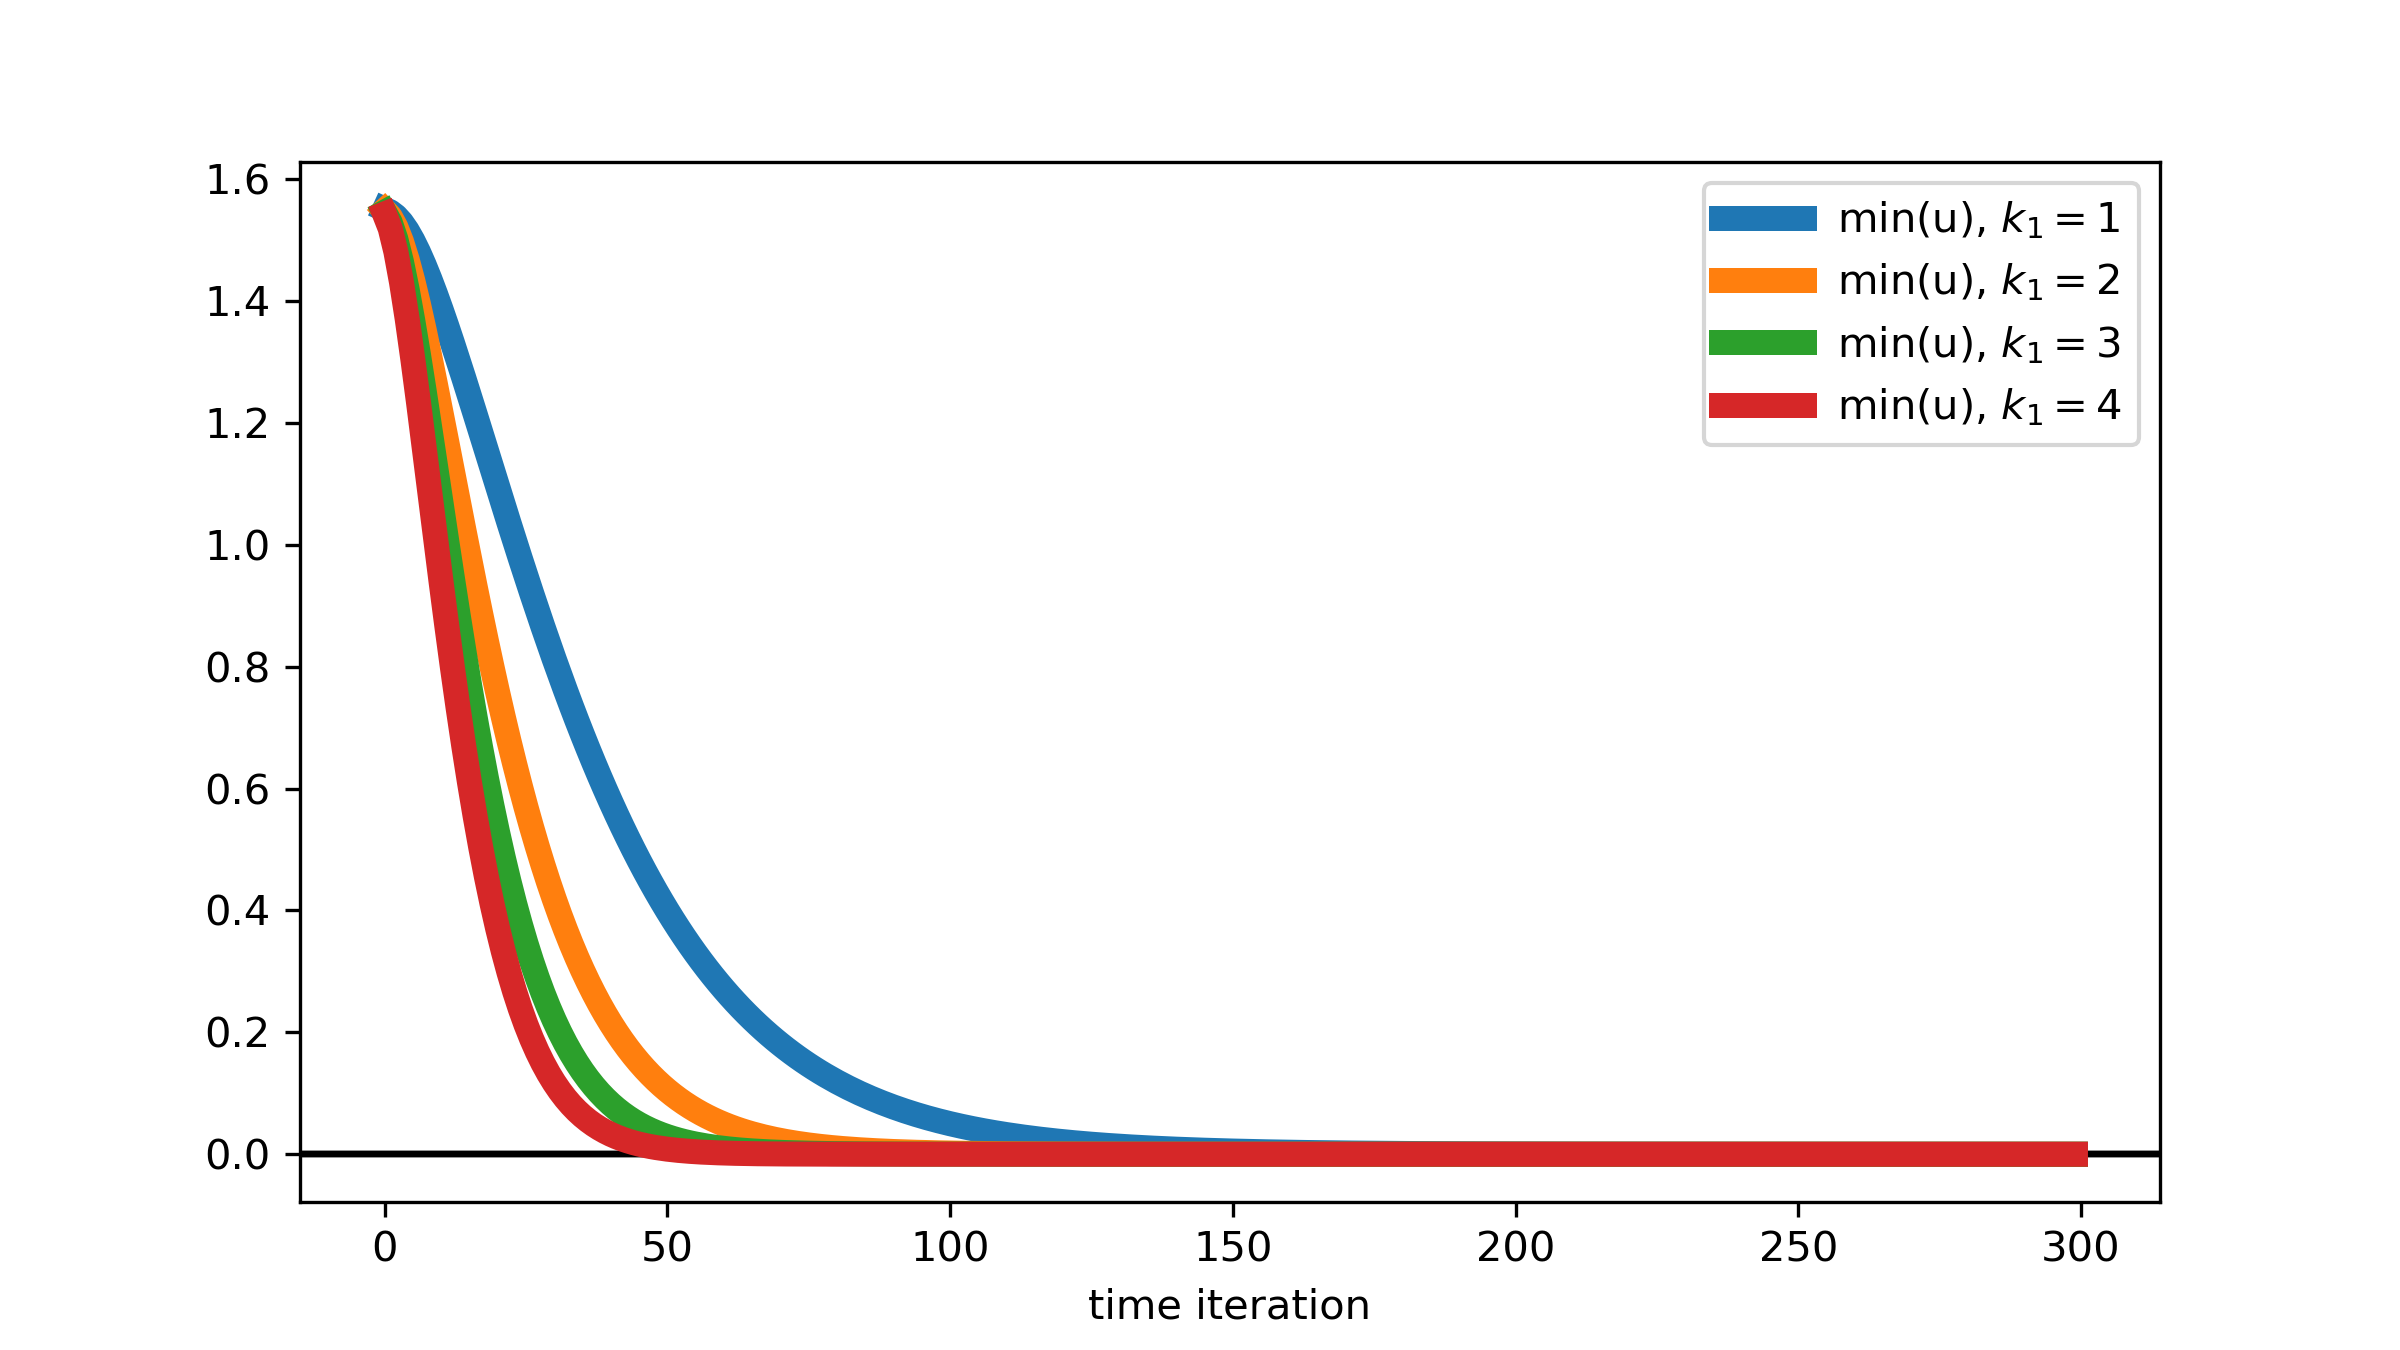
\includegraphics[width=0.8\textwidth]{positive_scheme_mass_k1=1,2,3,4.png}
          \par
          \small \alert{Implicit} scheme: mass conservation is
          \alert{{not satisfied}} for $u$, $k_2\in\{1,2,3,4\}$,
        \end{columns}
      \end{block}

      \begin{block}{Conclusions and Future Work}
        \small
        \begin{itemize}
        \item We have developed a \textbf{positive preserving} numerical scheme for classical Keller-Segel equations.
        \item It is based on (implicit and explicit) time scheme which \textbf{decouple calculus} of $u$ and $v$.
        \item \textbf{Discontinuous Galerkin} space approximation for cell density, $u$, FE approximation for chemical $v$.
        \item Future work: improve space approximation for $v$, \textbf{improve mass conservation}!!
        \end{itemize}
      \end{block}

    \end{column}

    \begin{column}{\sepmargin} \end{column}
  \end{columns}


  \vspace*{0.5cm}
  \begin{columns}[t]
    \begin{column}{\sepmargin}\end{column}
    \begin{column}{0.97\linewidth}
      {\color{blueMUW}\rule{1.012\textwidth}{10pt}}
    \end{column}
    \begin{column}{\sepmargin}\end{column}
  \end{columns}

  \vspace*{-1cm}
  \begin{columns}[t] % Split up the two columns wide column again

    \begin{column}{\sepmargin} \end{column}
    \begin{column}{\onecolwid}
      \begin{block}{\large References}
        \vspace*{-0.5cm}
        \nocite{*} % Insert publications even if they are not cited in the poster
        {\footnotesize
          % \bibliographystyle{plainurl}
          \bibliography{bibliog.bib}}
      \end{block}
    \end{column} % End of the second column
    \begin{column}{\sepwid}  \end{column}

    \begin{column}{\onecolwid}
      \begin{block}{\large Acknowledgement}
        \vspace*{-0.5cm}
        \footnotesize Second author is partially supported by the research group FQM-315 of Junta de Andalucı\'ia and by the project: New methods for predicting, manufacturing and application of shimming (FUTURE SHIMMING) -UIC AIRBUS, and the research team: Mathematics for Computational Intelligence Systems (M$\cdot$CIS).
      \end{block}
      \vspace*{-0.5cm}

      \begin{block}{\large Contact}
        \vspace*{-0.5cm}
        \footnotesize
        $^1$\emph{daniel.acostsoba@alum.uca.es}

        $^2$\emph{alba.navarroiz@alum.uca.es}

        $^3$\emph{rafael.rodriguez@uca.es}
      \end{block}
    \end{column}

    \begin{column}{\sepmargin}\end{column} % Empty spacer column



  \end{columns} % End of all the columns in the poster

\end{frame} % End of the enclosing frame

\end{document}
